\documentclass[conference]{IEEEtran}
\IEEEoverridecommandlockouts
% The preceding line is only needed to identify funding in the first footnote. If that is unneeded, please comment it out.
%Template version as of 6/27/2024

\usepackage{cite}
\usepackage{amsmath,amssymb,amsfonts}
\usepackage{algorithmic}
\usepackage{graphicx}
\usepackage{textcomp}
\usepackage{xcolor}
\usepackage[colorlinks=true, linkcolor=blue, urlcolor=blue]{hyperref}
\usepackage{minted}
\setminted{frame=lines, fontsize=\scriptsize, breaklines=true, linenos=false, autogobble=true}
\def\BibTeX{{\rm B\kern-.05em{\sc i\kern-.025em b}\kern-.08em
    T\kern-.1667em\lower.7ex\hbox{E}\kern-.125emX}}
\begin{document}

\title{Yelp Data Analysis - Phase I}

\author{\IEEEauthorblockN{Aayushi Pandey}
\IEEEauthorblockA{\textit{SEAS} \\
\textit{University at Buffalo}\\
Buffalo, NY, USA \\
\href{mailto:pandey25@buffalo.edu}{pandey25@buffalo.edu}}
\and
\IEEEauthorblockN{Om Nankar}
\IEEEauthorblockA{\textit{SEAS} \\
\textit{University at Buffalo}\\
Buffalo, NY, USA \\
\href{mailto:omnankar@buffalo.edu}{omnankar@buffalo.edu}}
\and
\IEEEauthorblockN{Sushrut Gaikwad}
\IEEEauthorblockA{\textit{SEAS} \\
\textit{University at Buffalo}\\
Buffalo, NY, USA \\
\href{mailto:sushruti@buffalo.edu}{sushruti@buffalo.edu}}
}

\maketitle

\begin{abstract}
This project focuses on building a big data pipeline using the Yelp Open Dataset,
which contains data about millions of reviews, business records, users, tips, and
checkins. In the first phase, we set up a Hadoop cluster and implement a Java-based
script to ingest the data. After ingestion, we carried out exploratory data analysis
using Python and pandas to uncover patterns in the data. We also identify three
potential machine learning use cases that can be solved using this data: sentiment
analysis of reviews, personalized recommendation system, and fake review detection.
Additionally, we defined five data analysis objectives to guide our exploratory
work. These early steps help lay the foundation for deeper modeling and insights
in later phases of the project.
\end{abstract}

\begin{IEEEkeywords}
Hadoop, Yelp Dataset, Data Ingestion, Exploratory Data Analysis, Machine Learning
\end{IEEEkeywords}

\section{Introduction}
Yelp is a popular online application that publishes crowd-sourced reviews about
businesses. Users can leave reviews, ratings, and tips about local businesses,
making it a rich source of large real-world data. Analyzing this data can reveal
insights about user preferences, business trends, regional patterns, and more.
However, working with such a large dataset calls for tools and systems that can
handle scale.

Our project aims to build a complete end-to-end big data pipeline to process and
analyze the Yelp Open Dataset. In this first phase, we focused on setting up the
infrastructure and preparing the data for analysis. We created a Hadoop cluster
on our local machine and wrote a Java-based script to ingest the data into the Hadoop
Distributed File System (HDFS). In parallel, we used Python and the pandas library
to carry out exploratory data analysis (EDA) to get familiar with the structure
of the data and uncover the basic trends.

In addition, we also outlined three potential machine learning problems: review
sentiment classification, recommendation systems, and fake review detection. We
also defined five data analysis objectives to study user behavior, business
popularity, and geographic patterns. These tasks gave us a better
understanding of the dataset and also set the direction for future phases, where
we plan to implement the machine learning methods and advanced analytics.

\section{Dataset Description}

As mentioned earlier, we are using the \href{https://business.yelp.com/data/resources/open-dataset/}{Yelp Open Dataset},
a publicly available collection of user generated data shared by Yelp for academic
purposes. It is a rich source of real-world data involving users, businesses, reviews,
and more. It is especially suitable for building end-to-end big data pipelines
and building machine learning models due to its size, structure, and variety.

\subsection{Individual Datasets}

The data is in the form of JSON files. The five main JSON files are the following:
\begin{itemize}
    \item \texttt{business.json}: It contains information about each business,
    such as name, location (city, state, latitude, longitude), star rating,
    number of reviews, categories, and various business attributes (e.g.,
    parking availability, takeout options).
    \item \texttt{review.json}: It includes full user-written reviews with
    associated star ratings, review dates, and metadata like the number of ``useful",
    ``funny", and ``cool" votes each review received.
    \item \texttt{user.json}: It provides metadata about users including number
    of reviews written, average star rating, number of fans, compliments received,
    and a list of friends (as user IDs).
    \item \texttt{checkin.json}: It records check-in activity on businesses, with
    timestamp data.
    \item \texttt{tip.json}: It is similar to reviews but shorter in length,
    these are quick suggestions or comments written by users for businesses.
\end{itemize}

Each file is stored in JSON format with one object per line. Such files can be
easily read using pandas by using the \texttt{read\_json} method. The entire data
is relatively large in size with millions of rows. Further, the data is also
relational. We can use columns like \texttt{user\_id} and \texttt{business\_id}
like keys to connect different JSON files.

Note that the \texttt{review.json} file was too large for us to load in our memory.
Hence we used a sample of the first 1,000,000 lines from this file and did EDA
on that.

\section{Exploratory Data Analysis}

Some insights that we have gathered using EDA are the following.

\subsection{Business Data}

The \texttt{business.json} file contains metadata more than 150,000 businesses,
including name, location, rating, and operational status.
\begin{itemize}
    \item \textbf{Geographical Insights:} Most businesses are located in Philadelphia,
    Pennsylvania, with over 1,400 unique cities and 27 states represented. Latitude
    and longitude distributions revealed distinct city clusters on the map.
    \item \textbf{Rating Distribution:} Star ratings are concentrated around 4.0, 
    and most businesses are still open (about 80\%).
    \item \textbf{Review Count:} The \texttt{review\_count} column showed an
    extremely heavy right skew, indicating a few highly-reviewed businesses and
    a long tail of lesser-reviewed ones.
    \item \textbf{Missing Values:} The \texttt{attributes} and \texttt{hours}
    columns had 9\% and 15.5\% missing values respectively, while \texttt{categories}
    had very few missing entries.
    \item \textbf{Multivariate Analysis:} Scatterplots and barplots suggested
    that businesses with more reviews tended to have slightly higher average
    ratings, but business status (open/closed) did not have a strong influence
    on average rating.
\end{itemize}

\subsection{Check-in Data}

The \texttt{checkin.json} file contains timestamped records of customer visits
to businesses. Each record corresponds to a business and includes a string of
check-in timestamps.
\begin{itemize}
    \item \textbf{Coverage:} Check-in data is available for approximately 38,000
    unique businesses, indicating a subset of all businesses in the dataset.
    \item \textbf{Total Check-ins:} By parsing the timestamp strings, we found
    the total number of check-ins to be approximately 1.9 million.
    \item \textbf{Data Quality:} The dataset contains no missing values, which
    makes it reliable for further analysis.
    \item \textbf{Potential Use:} Check-ins can be used in future work to analyze
    business popularity trends over time, identify peak business hours, or track
    seasonal patterns in customer engagement.
\end{itemize}

\subsection{Tip Data}

The \texttt{tip.json} file contains short, user-written comments about businesses.
Unlike reviews, tips are typically brief suggestions or remarks and are often
written in a more informal style.
\begin{itemize}
    \item \textbf{Content and Structure:} Each tip includes a \texttt{user\_id},
    \texttt{business\_id}, \texttt{text}, \texttt{date}, and a \texttt{compliment\_count},
    which indicates how many users complimented the tip.
    \item \textbf{Volume and Activity:} The number of tips steadily increased
    between 2011 and 2019, with the highest volume in 2012. Monthly tip volume
    appears to be evenly distributed, indicating consistent usage throughout the year.
    \item \textbf{User and Business Engagement:} The most active tip givers and
    the most ``tipped" businesses were identified, showing a similar skew to that
    of reviews---a small number of users contribute disproportionately.
    \item \textbf{Compliment Analysis:} The majority of tips received zero
    compliments, indicating that while tips are useful, they do not attract as
    much engagement as full reviews.
\end{itemize}

\subsection{User Data}

The \texttt{user.json} file provides rich metadata about individual Yelp users,
including review counts, average ratings, compliment types, and friend connections.
This data is essential for understanding user engagement and behavior on the
platform.
\begin{itemize}
    \item \textbf{User Growth Over Time:} The number of users steadily increased
    between 2011 and 2018, peaking in 2015. This trend reflects Yelp's growing
    popularity in that time period.
    \item \textbf{Review Counts:} The distribution of user review counts is highly
    right-skewed---most users have written only a few reviews, while a small number
    of users are extremely active.
    \item \textbf{Average Ratings:} Users tend to give high ratings, with the
    distribution of average stars centered around 4.0.
    \item \textbf{Social Network:} The majority of users have zero friends on the
    platform. This suggests that while Yelp includes social features, many users
    interact independently.
    \item \textbf{Compliment Analysis:} Compliment columns such as \texttt{compliment\_hot},
    \texttt{compliment\_funny}, and \texttt{compliment\_writer} are all highly
    correlated, suggesting that active or well-received users tend to be
    complimented in multiple ways.
    \item \textbf{Top Users:} We also identified the top-10 most complimented users
    and broke down their compliment types.
\end{itemize}

Instructions on how to run our EDA notebook is given in the Appendix, i.e.,
Section \ref{app:1}.

\section{System Setup}

The provided \texttt{docker-compose.yml} file is used for the Hadoop cluster setup
and the steps are followed using the \texttt{README.md} file. The main requirements
are to have Docker and Maven installed on the system, the installation check for
which can be verified using the two commands:
\begin{minted}{bash}
    docker --version
    # Output: Docker version 27.3.1, build ce12230
\end{minted}
\begin{minted}{bash}
    hadoop version
    # Output: 3.4.1
\end{minted}
Next, the following command starts the local Hadoop cluster inside Docker.
\begin{minted}{bash}
    docker compose -f docker-compose.yaml up -d
\end{minted}
Also, the NameNode, DataNode, ResourceManager, and NodeManager start in Docker.
Their creation and verification of whether they are running properly can be seen
from the screenshot shown in Figure \ref{fig:nodes_verification}.
\begin{figure*}[htbp]
    \centerline{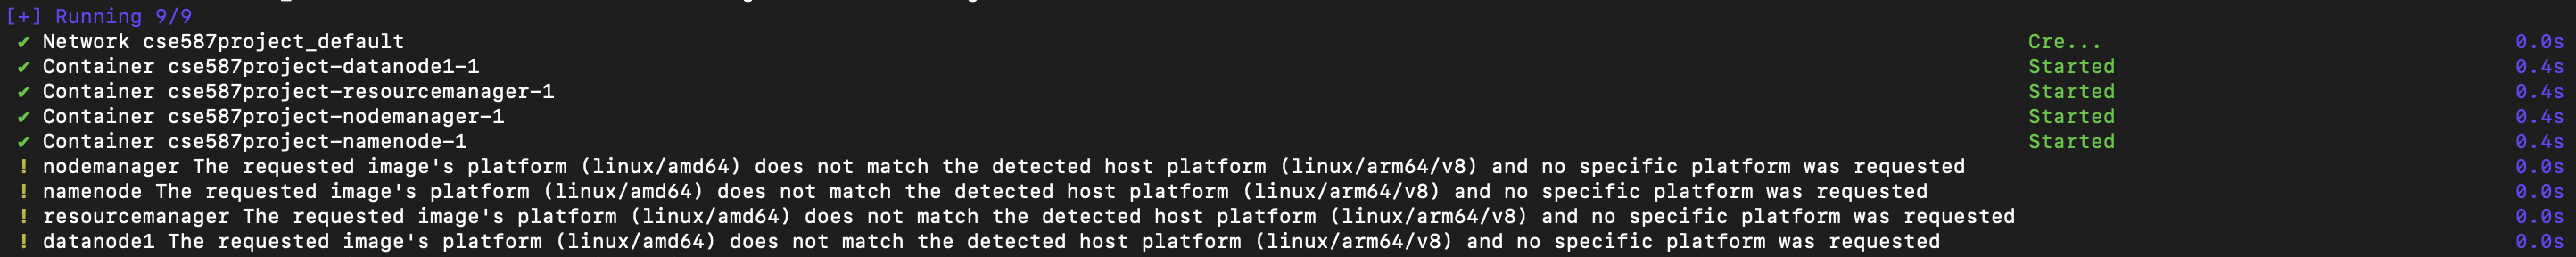
\includegraphics[width=1\textwidth]{graphics/nodes_verification.png}}
    \caption{Creation of NameNode, DataNode, ResourceManager, and NodeManager.}
    \label{fig:nodes_verification}
\end{figure*}
The Docker desktop application also shows the cluster. Its screenshot is shown
in Figure \ref{fig:docker_desktop}.
\begin{figure*}[htbp]
    \centerline{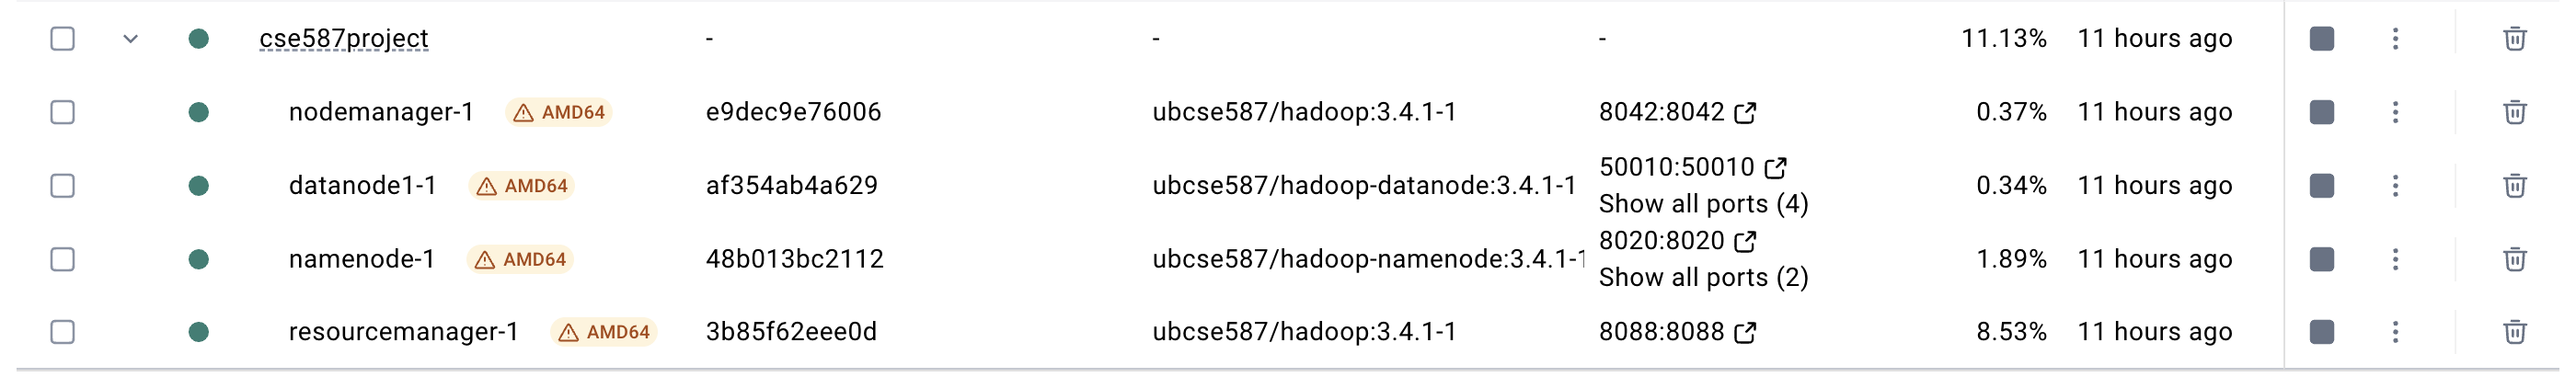
\includegraphics[width=1\textwidth]{graphics/docker_desktop.png}}
    \caption{Creation of NameNode, DataNode, ResourceManager, and NodeManager as
    shown by the Docker desktop application The green dot indicates that the
    containers are running properly.}
    \label{fig:docker_desktop}
\end{figure*}

Next, to test the system setup, we add a \texttt{README.txt} file which has the
following content:
\begin{minted}{bash}
    For the latest information about Hadoop, please visit our website at:
        http://hadoop.apache.org/
    and our wiki, at:
        https://cwiki.apache.org/confluence/display/HADOOP/
\end{minted}
This content is written to the NameNode using the following commands:
\begin{minted}{bash}
    docker exec -it project-namenode-1 bash
    hdfs dfs -mkdir /input
    hdfs dfs -put README.txt /input/wc.txt
\end{minted}
The first command is to get in the NameNode, the second is to create a directory
in the NameNode, and the third command creates a file \texttt{wc.txt} with the
content of \texttt{README.txt}.

The creation of the files and directories can be seen on \texttt{http://localhost:9870}.
The creation of the file can also be verified inside the terminal, as is shown
in Figure \ref{fig:verification_of_file_creation_in_terminal}.
\begin{figure}[htbp]
    \centerline{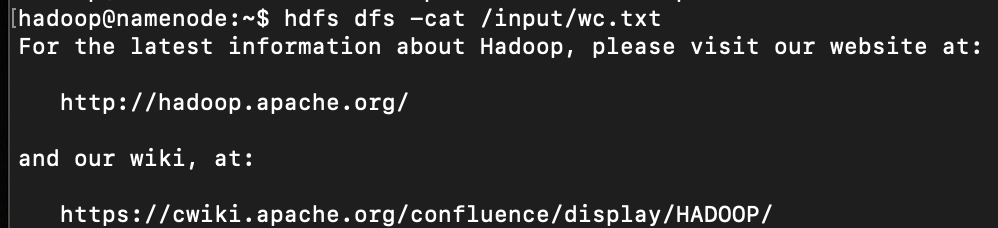
\includegraphics[width=0.48\textwidth]{graphics/verification_of_file_creation_in_terminal.png}}
    \caption{File creation shown in the terminal.}
    \label{fig:verification_of_file_creation_in_terminal}
\end{figure}

This confirms that the setup is successful and the Hadoop cluster is running.

\section{Data Ingestion}

Now, we will discuss how the Yelp dataset (JSON files) are ingested into the Hadoop
cluster that was setup in the previous section.

\subsection{Hadoop Installation and Verification}

Before beginning data ingestion, Hadoop was installed and its installation was
verified using the following command:
\begin{minted}{bash}
    hadoop version
    # Output: 3.4.1
\end{minted}
This command checks if Hadoop is correctly installed and configured by displaying
the installed version details.

\subsection{Maven Project Setup}

A Maven project was created with the structure shown in Figure \ref{fig:maven_structure}.
\begin{figure}[htbp]
    \centerline{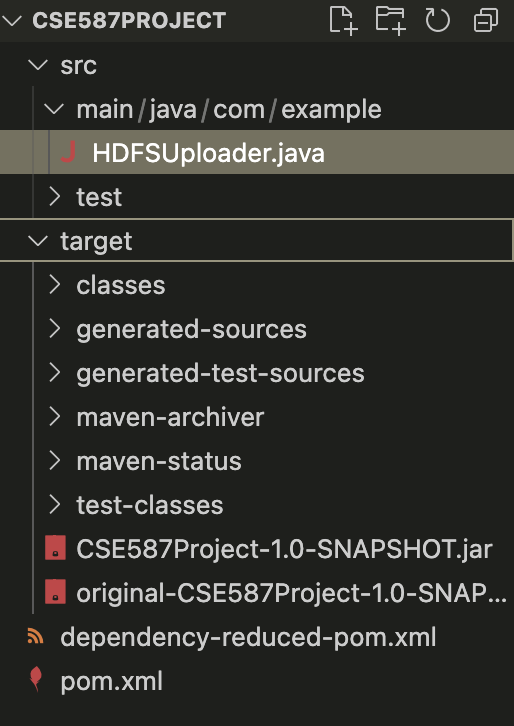
\includegraphics[width=0.28\textwidth]{graphics/maven_structure.png}}
    \caption{Maven project structure.}
    \label{fig:maven_structure}
\end{figure}
The \texttt{pom.xml} file contains the necessary dependencies for Hadoop, Woodstox
(XML parser), and the Maven Shade Plugin for packaging the project as a JAR file.
The dependencies include:
\begin{itemize}
    \item \texttt{hadoop-common}
    \item \texttt{hadoop-hdfs}
    \item \texttt{hadoop-client}
    \item \texttt{hadoop-mapreduce-client-core}
    \item \texttt{hadoop-yarn-client}
    \item \texttt{woodstox-core}
\end{itemize}
The content of the \texttt{pom.xml} file is the following:
\begin{minted}{xml}
<?xml version="1.0" encoding="UTF-8"?>
<project xmlns="http://maven.apache.org/POM/4.0.0" xmlns:xsi="http://www.w3.org/2001/XMLSchema-instance" xsi:schemaLocation="http://maven.apache.org/POM/4.0.0 http://maven.apache.org/maven-v4_0_0.xsd">
  <modelVersion>4.0.0</modelVersion>
  <groupId>com.example</groupId>
  <artifactId>CSE587Project</artifactId>
  <packaging>jar</packaging>
  <version>1.0-SNAPSHOT</version>
  <name>CSE587Project</name>
  <url>http://maven.apache.org</url>
  <dependencies>
    <!-- Hadoop Common -->
    <dependency>
      <groupId>org.apache.hadoop</groupId>
      <artifactId>hadoop-common</artifactId>
      <version>3.4.1</version>
      <!-- Ensure this matches your Hadoop version -->
    </dependency>
    <!-- Hadoop HDFS -->
    <dependency>
      <groupId>org.apache.hadoop</groupId>
      <artifactId>hadoop-hdfs</artifactId>
      <version>3.4.1</version>
    </dependency>
    <!-- Hadoop Client -->
    <dependency>
      <groupId>org.apache.hadoop</groupId>
      <artifactId>hadoop-client</artifactId>
      <version>3.4.1</version>
    </dependency>
    <!-- Woodstox Core (StAX XML parser) -->
    <dependency>
      <groupId>com.fasterxml.woodstox</groupId>
      <artifactId>woodstox-core</artifactId>
      <version>6.4.0</version>
    </dependency>
    <!-- Hadoop MapReduce Client (if needed) -->
    <dependency>
      <groupId>org.apache.hadoop</groupId>
      <artifactId>hadoop-mapreduce-client-core</artifactId>
      <version>3.4.1</version>
    </dependency>
    <!-- Hadoop Yarn Client (if needed) -->
    <dependency>
      <groupId>org.apache.hadoop</groupId>
      <artifactId>hadoop-yarn-client</artifactId>
      <version>3.4.1</version>
    </dependency>
    <dependency>
      <groupId>org.apache.hadoop</groupId>
      <artifactId>hadoop-hdfs-client</artifactId>
      <version>3.4.1</version>
      <!-- Ensure it matches your Hadoop version -->
    </dependency>
    <!-- Hadoop Client API -->
    <dependency>
      <groupId>org.apache.hadoop</groupId>
      <artifactId>hadoop-client-api</artifactId>
      <version>3.4.1</version>
    </dependency>
    <!-- Hadoop Client Runtime -->
    <dependency>
      <groupId>org.apache.hadoop</groupId>
      <artifactId>hadoop-client-runtime</artifactId>
      <version>3.4.1</version>
    </dependency>
  </dependencies>
  <build>
    <plugins>
      <plugin>
        <groupId>org.apache.maven.plugins</groupId>
        <artifactId>maven-shade-plugin</artifactId>
        <version>3.2.4</version>
        <executions>
          <execution>
            <phase>package</phase>
            <goals>
              <goal>shade</goal>
            </goals>
            <configuration>
              <filters>
                <filter>
                  <artifact>*:*</artifact>
                  <excludes>
                    <exclude>META-INF/*.SF</exclude>
                    <exclude>META-INF/*.DSA</exclude>
                    <exclude>META-INF/*.RSA</exclude>
                  </excludes>
                </filter>
              </filters>
            </configuration>
          </execution>
        </executions>
      </plugin>
    </plugins>
  </build>
</project>
\end{minted}

\subsection{Java Script for HDFS Upload}

The \texttt{HDFSUploader.java} script uploads the local Yelp JSON files to HDFS.
The script does the following:
\begin{enumerate}
    \item Establishes a connection to HDFS.
    \item Ensures that the destination directory exists.
    \item Iterates over the local dataset directory to find the JSON files.
    \item Checks the existence of the file to avoid redundancy.
    \item Copies the JSON files to HDFS.
\end{enumerate}
The content of the \texttt{HDFSUploader.java} is the following:
\begin{minted}{java}
package com.example;

import org.apache.hadoop.conf.Configuration;
import org.apache.hadoop.fs.FileSystem;
import org.apache.hadoop.fs.Path;
import org.apache.hadoop.fs.FileStatus;
import java.io.File;
import java.io.IOException;
import java.net.URI;

public class HDFSUploader {
    public static void main(String[] args) {
        // Local directory containing Yelp JSON files
        //String localDir = "/Users/omnankar/Documents/Spring sem/CSE 587/CSE587project/Yelp JSON/yelp_dataset/";
        String localDir = "/tmp/yelp_dataset/";
        String hdfsDestination = "/yelp_dataset/";

        try {
            // Load Hadoop Configuration
            Configuration conf = new Configuration();
            conf.set("fs.defaultFS", "hdfs://namenode:8020"); // Or use the actual Namenode IP
            conf.set("fs.hdfs.impl", "org.apache.hadoop.hdfs.DistributedFileSystem");
            conf.set("fs.file.impl", "org.apache.hadoop.fs.LocalFileSystem");

            // Initialize HDFS FileSystem
            FileSystem fs = FileSystem.get(new URI("hdfs://namenode:8020"), conf);

            // Ensure destination directory exists
            Path hdfsDestPath = new Path(hdfsDestination);
            if (!fs.exists(hdfsDestPath)) {
                fs.mkdirs(hdfsDestPath);
                System.out.println("Created HDFS directory: " + hdfsDestination);
            }

            // Get list of files to upload
            File folder = new File(localDir);
            File[] listOfFiles = folder.listFiles((dir, name) - > name.endsWith(".json"));

            if (listOfFiles == null || listOfFiles.length == 0) {
                System.out.println("No JSON files found in local directory: " + localDir);
                return;
            }

            // Upload each file
            for (File file: listOfFiles) {
                Path srcPath = new Path(file.getAbsolutePath());
                Path destPath = new Path(hdfsDestination + file.getName());

                // Check if file already exists in HDFS
                if (fs.exists(destPath)) {
                    System.out.println("Skipping (already exists): " + file.getName());
                    continue;
                }

                // Upload file
                fs.copyFromLocalFile(srcPath, destPath);
                System.out.println("Uploaded: " + file.getName());
            }

            fs.close();
            System.out.println("All files uploaded successfully!");

        } catch (Exception e) {
            System.err.println("Error uploading files to HDFS: " + e.getMessage());
            e.printStackTrace();
        }
    }
}
\end{minted}

\subsection{Execution Steps}

\subsubsection{Copy Yelp Dataset To NameNode Container}

\begin{minted}{bash}
docker cp "/local/path/to/yelp_dataset" cse587project-namenode-1:/tmp/yelp_dataset
\end{minted}
This copies the dataset from the local system into the Docker container where the
NameNode is running.

\subsubsection{Build the Maven Project}

\begin{minted}{bash}
mvn clean package
\end{minted}
This compiles the Java code and packages it as a JAR file. The JAR file
(\texttt{CSE587Project-1.0-SNAPSHOT.jar}) contains the compiled Java code for
the script which was run. It is responsible for uploading Yelp dataset JSON
files to HDFS.

\subsubsection{Copy JAR File to NameNode Container}

\begin{minted}{bash}
docker cp target/CSE587Project-1.0-SNAPSHOT.jar cse587project-namenode-1:/tmp/
\end{minted}
This is shown in Figure \ref{fig:successfully_copied}.
\begin{figure*}[htbp]
    \centerline{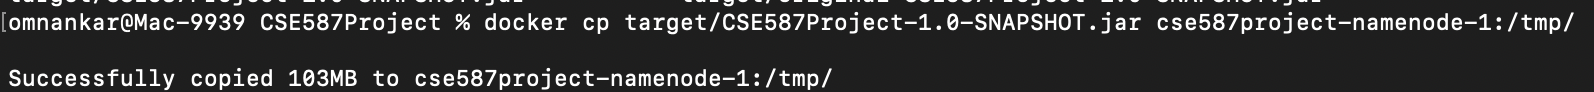
\includegraphics[width=1\textwidth]{graphics/successfully_copied.png}}
    \caption{Copying JAR file to NameNode container.}
    \label{fig:successfully_copied}
\end{figure*}
This moves the compiled JAR file into the NameNode container for execution.

\subsubsection{Run HDFSUploader Inside NameNode Container}

\begin{minted}{bash}
docker exec -it cse587project-namenode-1 bash -c 'java -cp /tmp/CSE587Project-1.0-SNAPSHOT.jar com.example.HDFSUploader'
\end{minted}
This is shown in Figure \ref{fig:successfully_copied_9_29}.
\begin{figure*}[htbp]
    \centerline{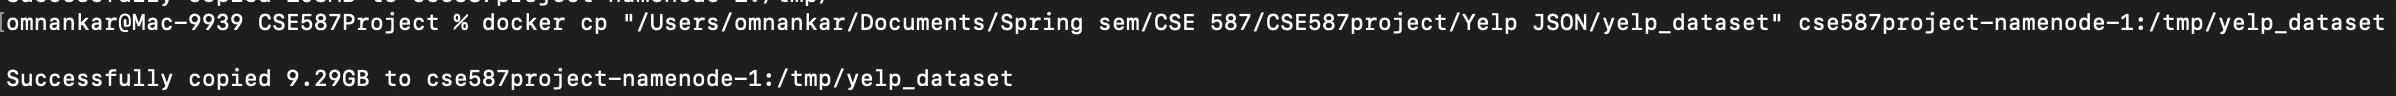
\includegraphics[width=1\textwidth]{graphics/successfully_copied_9_29.png}}
    \caption{Running HDFSUploader inside NameNode Container.}
    \label{fig:successfully_copied_9_29}
\end{figure*}
This executes the \texttt{HDFSUploader} Java program inside the Hadoop container
to upload data to HDFS.

\subsubsection{Verify Uploaded Files}

\begin{minted}{bash}
docker exec -it cse587project-namenode-1 bash -c 'hdfs dfs -ls /yelp_dataset'
\end{minted}
This is shown in Figure \ref{fig:verify_uploaded_files}.
\begin{figure*}[htbp]
    \centerline{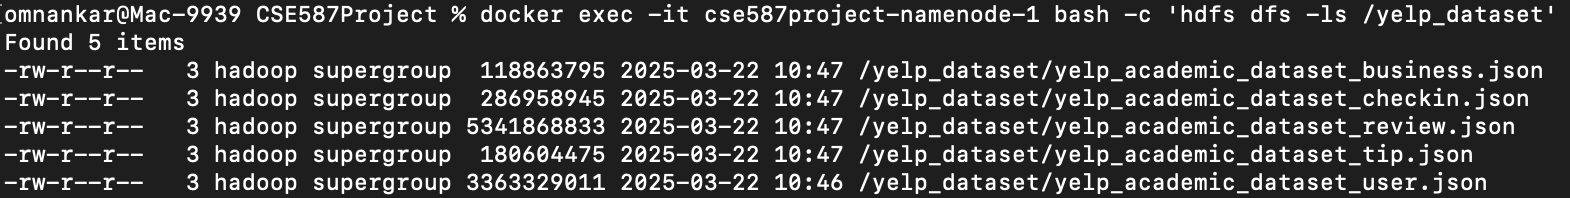
\includegraphics[width=1\textwidth]{graphics/verify_uploaded_files.png}}
    \caption{Verification of uploaded files.}
    \label{fig:verify_uploaded_files}
\end{figure*}

\subsection{Web Interface Verification}

The uploaded files were also verified using the Hadoop NameNode Web UI at
\texttt{http://localhost:9870}, where the \texttt{yelp\_dataset} directory and
its JSON files are visible. This is shown in Figures \ref{fig:root_dir} and
\ref{fig:yelp_dataset_dir}.
\begin{figure}[htbp]
    \centerline{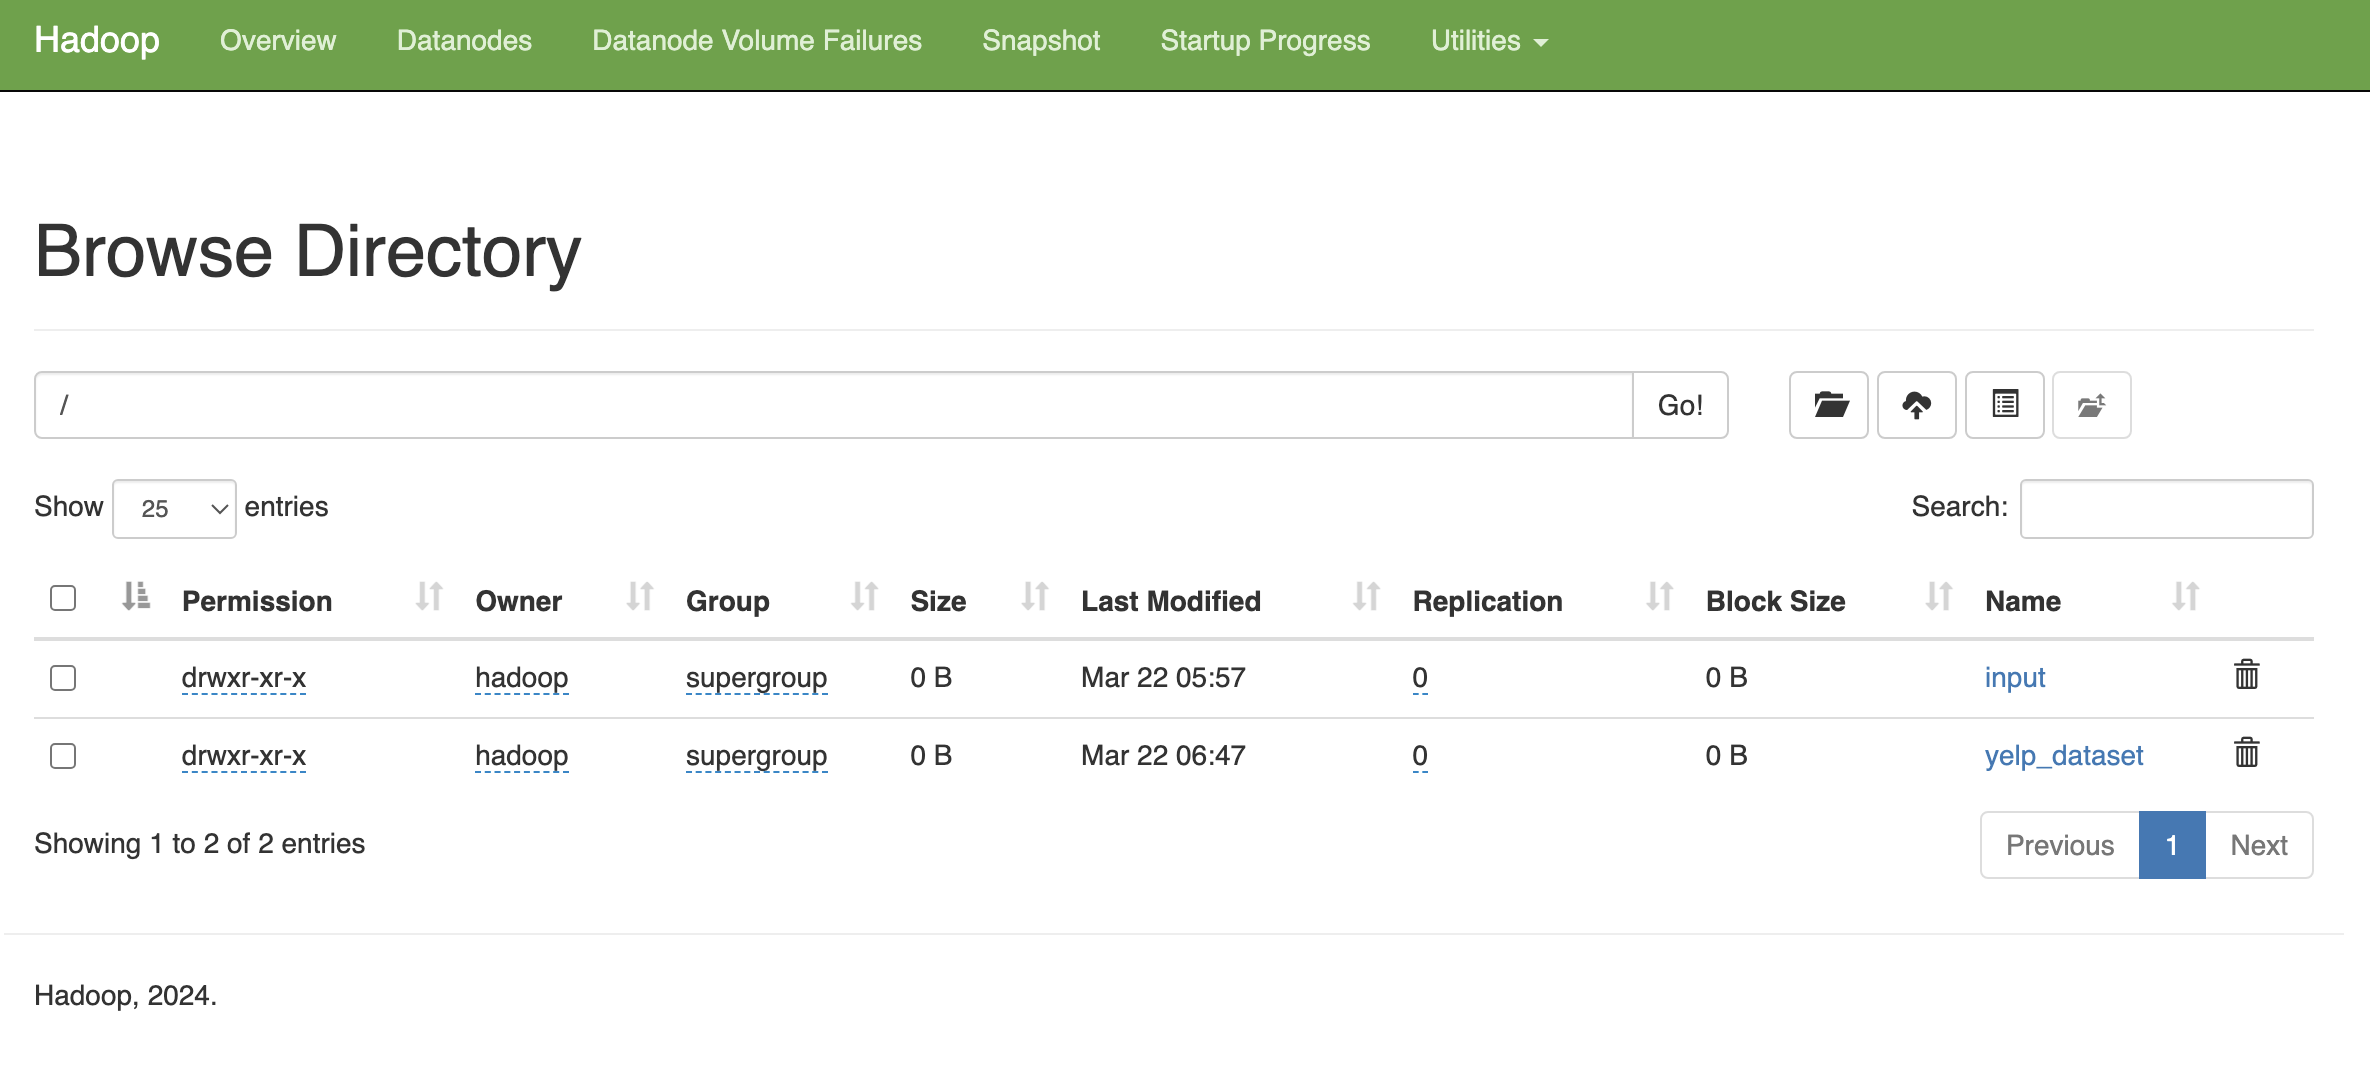
\includegraphics[width=0.48\textwidth]{graphics/root_dir.png}}
    \caption{Web interface verification of the root directory.}
    \label{fig:root_dir}
\end{figure}
\begin{figure}[htbp]
    \centerline{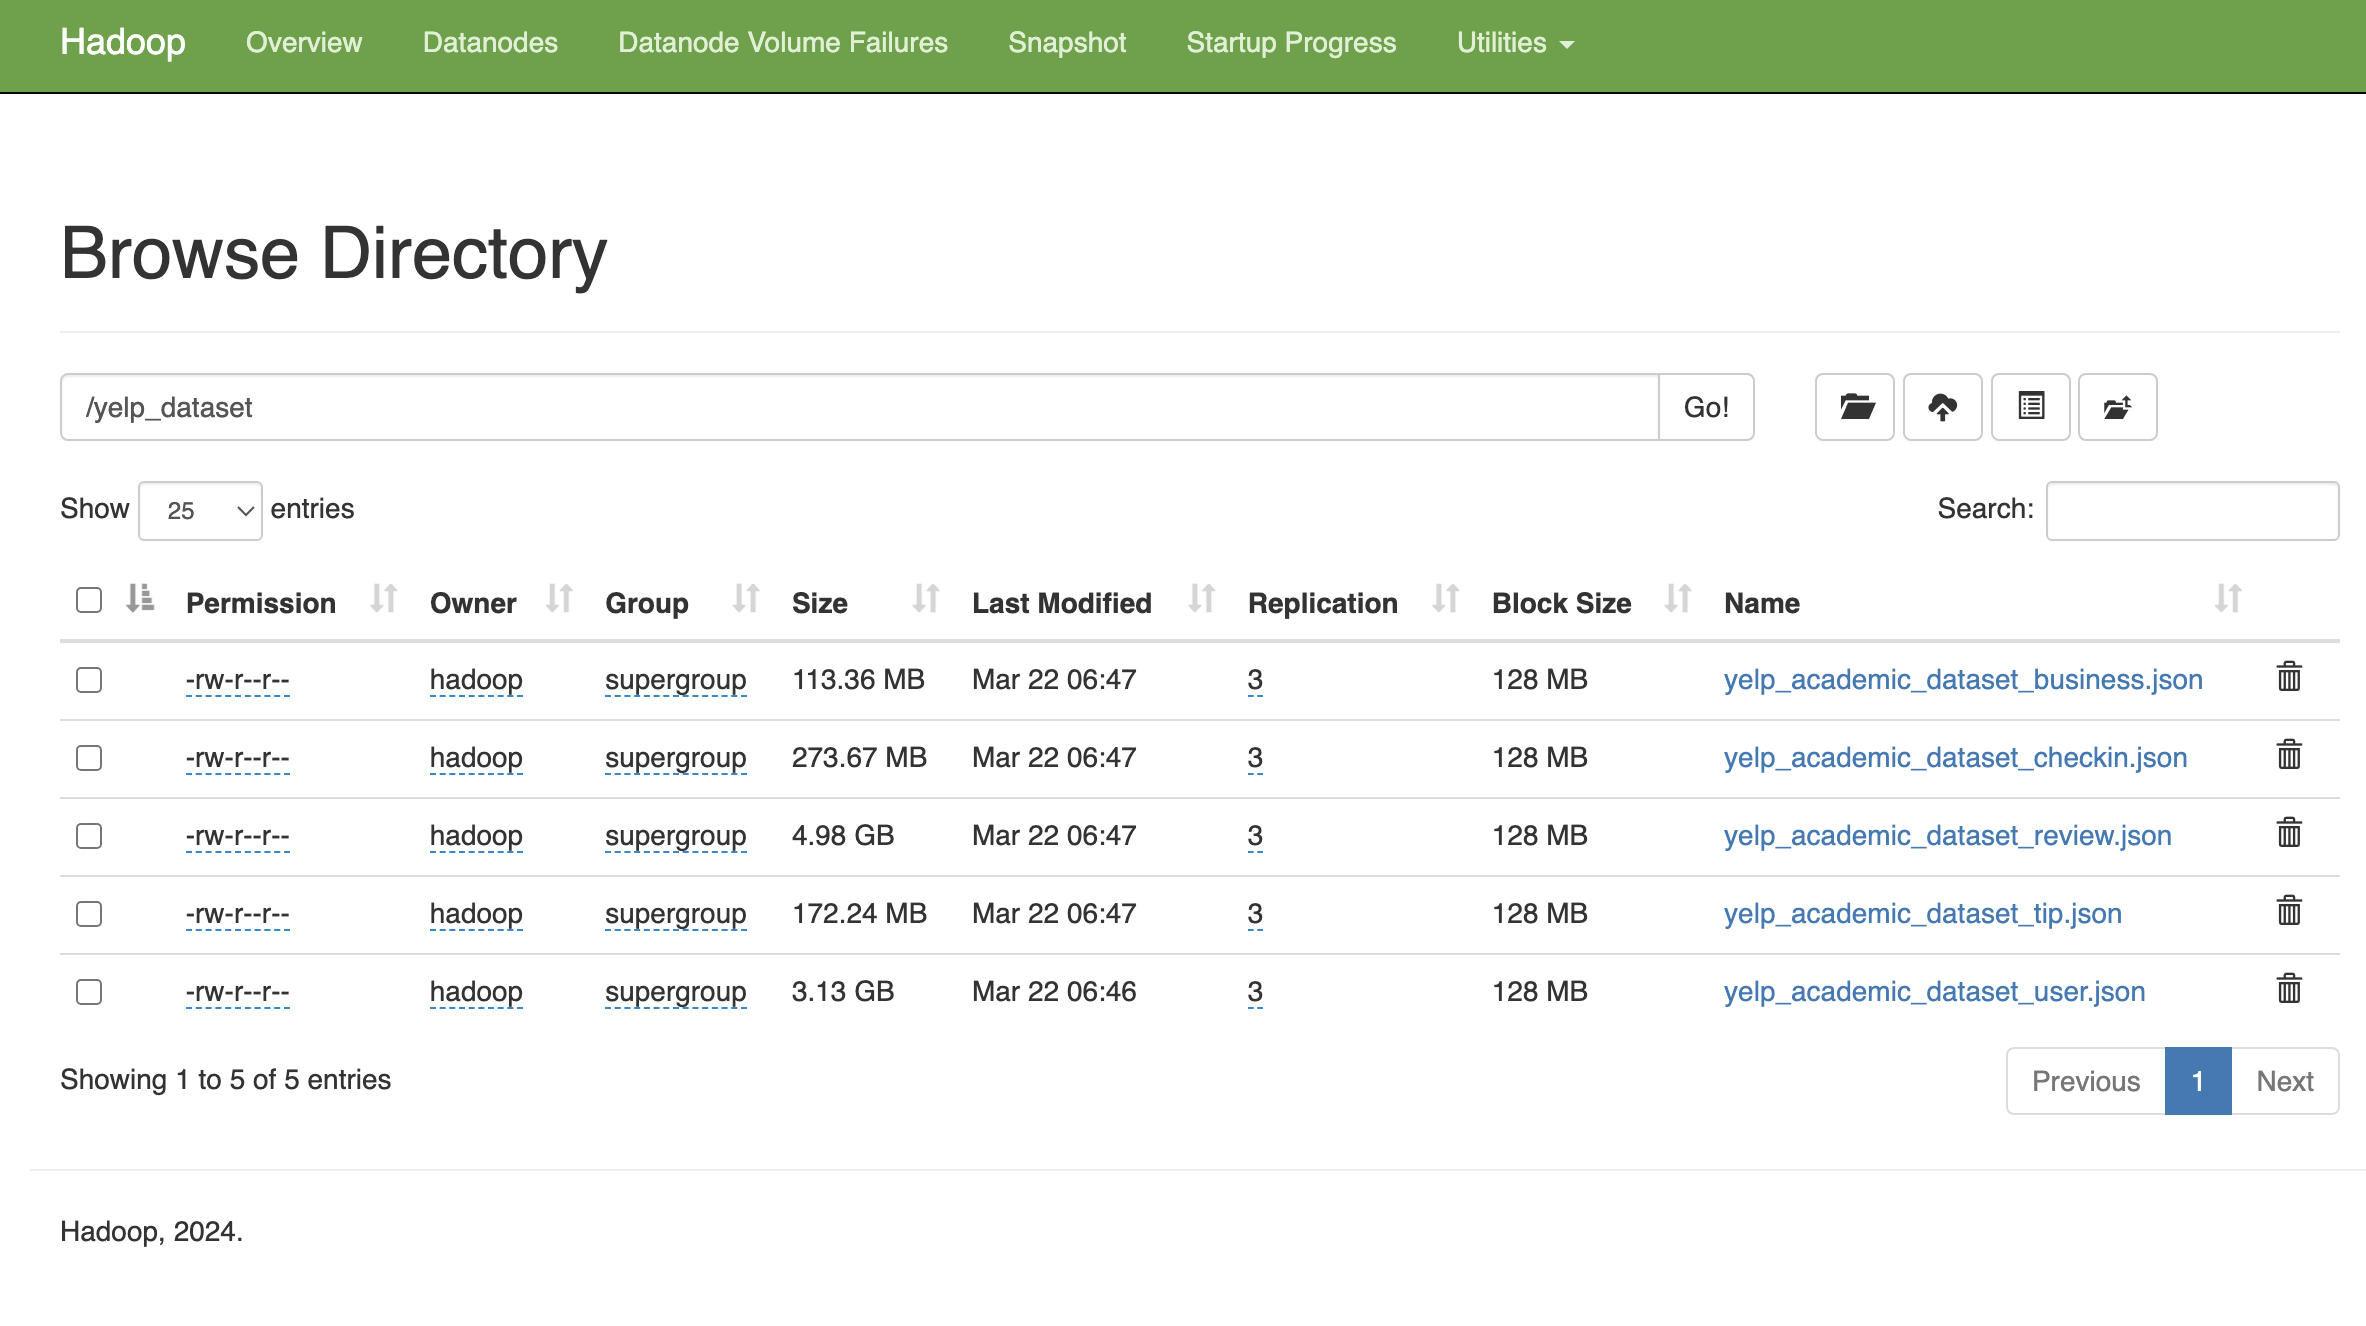
\includegraphics[width=0.48\textwidth]{graphics/yelp_dataset_dir.png}}
    \caption{Web interface verification of the \texttt{yelp\_dataset} directory.}
    \label{fig:yelp_dataset_dir}
\end{figure}

Another check is to read a few lines from the uploaded data. The first 5 lines
of the \texttt{business.json} file are read using the following command:
\begin{minted}{bash}
docker exec -it cse587project-namenode-1 bash -c 'hdfs dfs -cat /yelp_dataset/yelp_academic_dataset_business.json | head -n 5'
\end{minted}
Figure \ref{fig:verify_by_printing} shows the output.
\begin{figure*}[htbp]
    \centerline{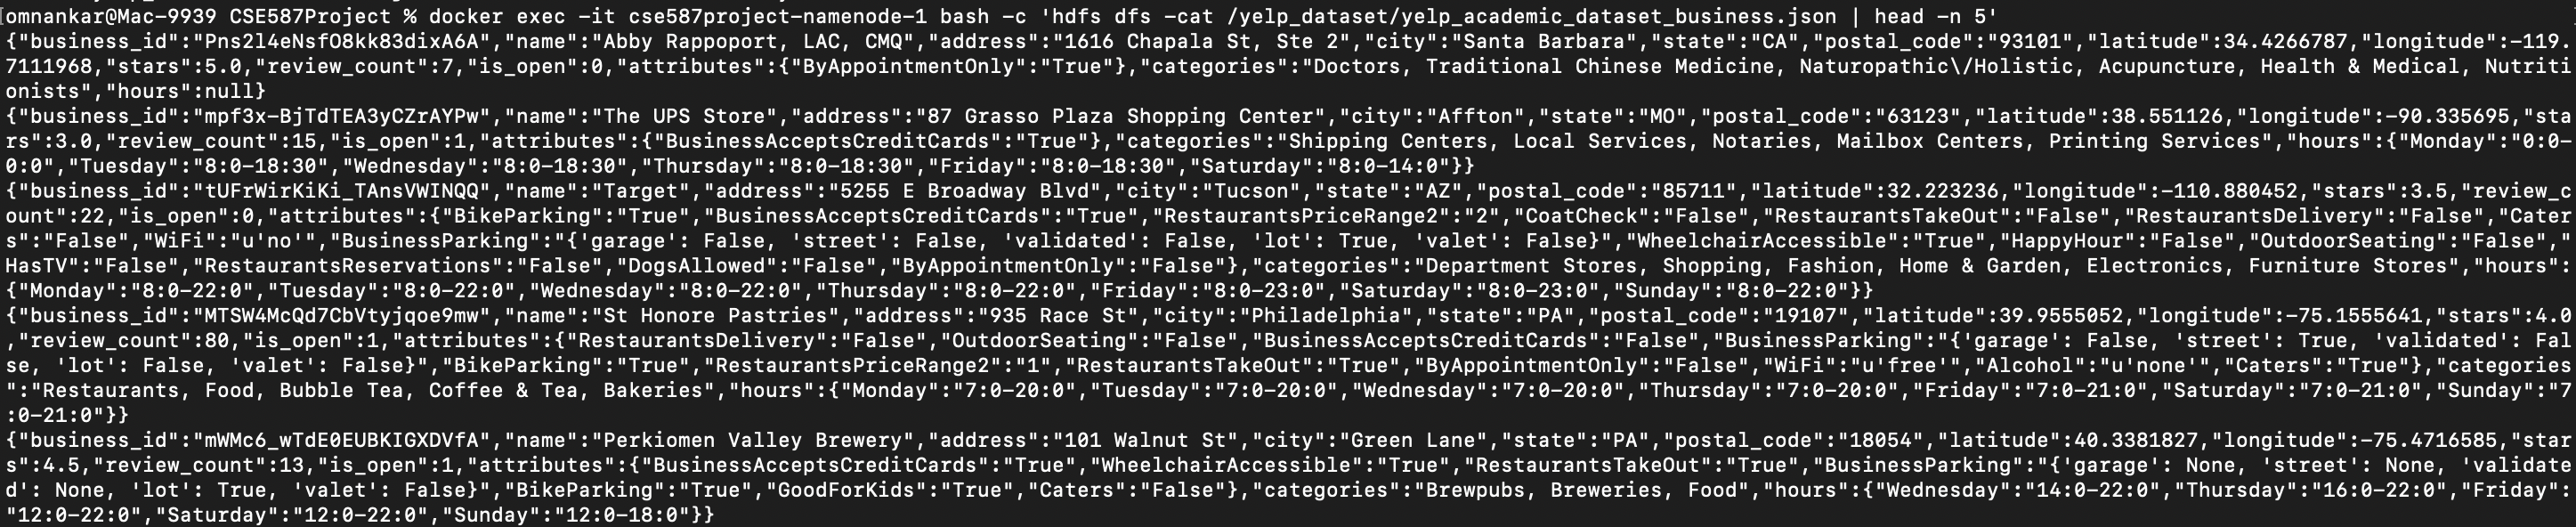
\includegraphics[width=1\textwidth]{graphics/verify_by_printing.png}}
    \caption{Verification by printing the first 5 lines of the \texttt{business.json}
    file.}
    \label{fig:verify_by_printing}
\end{figure*}

\subsection{Discussion on Data Ingestion Methods}

\subsubsection{Is \texttt{hdfs dfs -put} a good way to write files to an HDFS
cluster?}

Writing with \texttt{hdfs dfs -put} is a good way to write files into an HDFS
cluster for small- to medium-sized files and one time or spaced uploads. It is
simple, well-proven, and requires less commands. But if massive data ingestion
or bulk uploading is required, as in the case of uploading the Yelp dataset
(more than 9 GB) it may not be ideal due to its single-threaded approach and lack
of advanced features like compression or multi-threaded uploading.

\subsubsection{How to improve \texttt{hdfs dfs -put} speed?}

The speed on \texttt{hdfs dfs -put} while writing \texttt{README.txt} file to
input directory was satisfactory and quick but for data ingestion it will be very
slow. Some ways of improving it include:
\begin{itemize}
    \item Use the \texttt{-p} parameter for parallel copying.
    \item Increase the replication factor temporarily during upload (default is 3).
    \item Implement a custom solution using the HDFS API for parallel uploads.
\end{itemize}

\subsubsection{Best Data Formats for HDFS Storage}

Some formats to store data in HDFS for easy analysis afterwards are:
\begin{itemize}
    \item \textit{Parquet:} Columnar storage file format that uses effective
    compression and encoding schemes, often used when Excel or CSV file reach
    their row limit.
    \item \textit{JSON:} For semi-structured data, especially when human readability
    is essential.
\end{itemize}

The choice of format primarily depends on the specific analysis needs, query patterns,
and the tools which will be used to analyze the data.

\section{Machine Learning Problem Statements}

Based on our exploration of the Yelp Open Dataset, we came up with three machine
learning problems that not only fit well with the data but also address real-world
use cases. These problems aim to improve user experience and enhance the
trustworthiness of the platform.

\subsection{Sentiment Analysis of User Reviews}

The goal here is to predict the sentiment of a review---whether it is positive,
neutral, or negative---based on the review text. While the dataset already includes
star ratings, this task helps extract deeper insight from the actual text users
write. Sometimes, the sentiment expressed in the review does not match the star
rating, so this can give businesses a clearer picture of how customers feel. This
is a classic text classification problem that can be solved using supervised
learning, where the review text is used as input and the rating (or derived
sentiment label) is the target.

\subsection{Business Recommendation System}

We aim to build a recommendation system that suggests businesses to users based
on their past activity---mainly the reviews they have written and the ratings
they have given. This could help users discover new places they have likely to
enjoy, making the platform more useful and personalized. We can approach this
using collaborative filtering (based on user-item interactions), content-based
filtering (using business attributes), or a hybrid of both.

\subsection{Detecting Fake or Spam Reviews}

Another problem we identified is the detection of fake or suspicious reviews.
Some reviews may be overly positive or negative in a way that does not align with
a user's history or the overall business reputation. Spotting these can improve
the credibility of the platform and help users trust the information they see.
This can be treated as an anomaly detection or binary classification problem,
depending on how we define and label fake reviews. We can use features like review
text, timing, voting patterns, and user behavior to train a model that flags
potentially fake reviews.

\section{Data Analysis Objectives}

We have also defined five key objectives that will guide our deeper exploration of
the Yelp Open Dataset. These objectives are designed to help us uncover trends,
patterns, and relationships that can add value to both users and businesses on
the platform. The insights gained from these analyses will also help support
and validate our proposed machine learning tasks.

\subsection{User Trend Analysis}

We plan to study how the user base on Yelp has grown and evolved over time. By
analyzing the \texttt{yelping\_since} field in the \texttt{user.json} file, we
will track the number of new users joining the platform each year. This will help
us identify growth patterns and understand how user engagement has shifted across
different time periods.

\subsection{Business Category Performance}

We aim to evaluate how different categories of businesses perform in terms of
user engagement and satisfaction. Using data from \texttt{business.json}, including
the \texttt{categories}, \texttt{review\_count}, and \texttt{stars} fields, we
will identify the most reviewed categories and compare their average ratings.
This analysis will help us understand which types of businesses tend to attract
more user attention and how they are perceived by customers.

\subsection{User Engagement Patterns}

Another key objective is to investigate how frequently users contribute to the
platform and how that engagement influences their perceived credibility. We will
analyze \texttt{review\_count}, \texttt{average\_stars}, and compliment-related
metrics from the \texttt{user.json} file, alongside voting patterns from
\texttt{review.json}. This will allow us to distinguish between casual and highly
active users and assess their influence within the community.

\subsection{Geographic Distribution of Businesses}

We also plan to explore the geographic distribution of Yelp activity. By visualizing
the latitude and longitude coordinates in the \texttt{business.json} file, we
will identify which cities or regions have the highest concentration of reviewed
businesses. This spatial analysis will give us a clearer picture of Yelp's reach
and user engagement across different locations.

\subsection{Relationship Between Review Length and Rating}

Finally, we want to examine whether there is a connection between the length of
a review and the sentiment it conveys. In this analysis, we will compare the
character count of reviews (\texttt{text} field) with the corresponding star
ratings from the \texttt{review.json} file. This will help us understand if longer
reviews tend to reflect stronger opinions—either positive or negative—which can
be useful for both sentiment analysis and review quality assessment.

\section*{Appendix: Running the EDA Notebook}\label{app:1}

We have created an Anaconda environment for EDA. The \texttt{environment.yml} file
for our environment is provided in our submission. Please follow these steps to
run our EDA notebook:
\begin{enumerate}
    \item Using Anaconda prompt, navigate into the root directory (i.e., the
    directory you get after unzipping our submission).
    \item Create an environment using our \texttt{environment.yml} file by running
    the following commands in the Anaconda prompt:
    \begin{minted}{bash}
        conda create -p ./venv --file environment.yml
    \end{minted}
    \item The environment will be created in this root directory, inside the
    folder \texttt{venv}. Once this is done, activate this environment by running
    the following command:
    \begin{minted}{bash}
        conda activate ./venv
    \end{minted}
    \item Now, run the following command to open a Jupyter notebook server:
    \begin{minted}{bash}
    jupyter notebook
    \end{minted}
    Once this server opens, you can click on our submitted EDA notebook to open
    it.
\end{enumerate}

\end{document}
